\documentclass[10pt, twoside]{article}
\usepackage{be-my-concrete, be-my-geometry}
\usepackage{extra-algebra}
\setcounter{MaxMatrixCols}{15}

\begin{document}

\pagestyle{empty}
\begin{abstract}
    Физика — это бро матана, они вечно в тандемусе. Иногда физика ваще обгоняет матан по школьным левелам!!1
    Чтобы решать труЪ-задачки про бруски, маятники и прочее, надо уметь юзать скиллы типа дифференцируй тут и интегрируй там. На курсе мы станем джедаями матанализа: апгрейднем технику, разберёмся, как с физического на математический перевести, и вообще будем решать мощ-щ-щные штуки. 
    
    Будет больно, но весело!
\end{abstract}

\begin{figure}[h!]
    \centering
    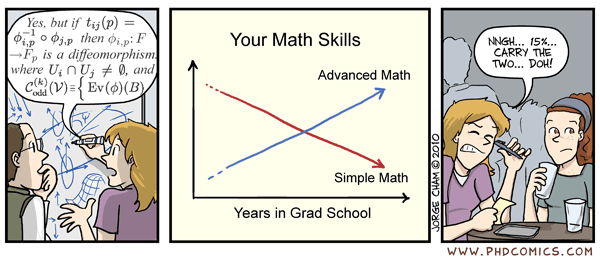
\includegraphics[width=0.8\textwidth]{pics/phd_comics.png}
\end{figure}
\newpage

\tableofcontents
\newpage

\setcounter{page}{1}
\pagestyle{fancy}
%советы для подопечных
\section*{Советы для семинаристов}
\addcontentsline{toc}{section}{Советы для семинаристов}

Часть этого руководства взята из плана к курсу Никиты Астраханцева (2017 год). Сами же советы были сформулированы Артемом Абановым. Были добавлены некоторые дополнения.
\begin{itemize}
    \item В начале каждого семинара делать наставления для школьников (2-3 минуты). Рассказать какую-нибудь байку или анекдот. 
    \item Школьники делятся на разные команды (столы) по их уровню знаний. Нужно сделать так, чтобы до школьника было близко идти, чтобы успеть поработать с каждым за вашим столом.
    \item Готовтесь к каждому семинару!!! Подумайте над задачами, которые вы можете дать конкретному школьнику, помимо заранее подготовленных. Сделайте это таким образом, чтобы вы их быстро могли вспомнить: сделайте распечатку, перепишите в тетрадь.
    \item Ваша задача - подобрать задачу уровня, немногим выше уровня школьника, чтобы ему/ей было комфортно, удобно и процесс был продуктивным.
    \item Если школьник решил задачу, то следует сделать следующее: 
    \begin{enumerate}
        \item Похвалить
        \item Проверить размерность/знак/ответ
        \item Обсудить предельные случаи. Поговорить о физике этих предельных случаев.
    \end{enumerate}
    \item Если задача у школьника вызывает затруднения, то стоит его подбодрить и помочь коротким советом.
    \item Если затруднения продолжаются, то стоит дать другую задачу, которая подведет к нерешенной задаче.
    \item Если видите, что школьники устали - рассказать байку/анекдот в тему занятия. 
    \item Всегда старайтесь добиться от школьника физического смысла, заложенного в формулах. Формулы - отражение физики задачи! 
\end{itemize}
\newpage
%первое занятие
\section{Функции одной переменной}
\epigraph{\textsf{Fear is the path to the dark side. Fear leads to anger, anger leads to hate, hate leads to suffering.}}{\texttt{Yoda}}
\paragraph{Зачем нам нужны функции?} Так исторически сложилось, что физические законы плохо интерпретируемы без использования какого-то вспомогательного аппарата/языка, который 
позволяет нам записывать эти законы. Функции - это один из таких языков, который позволяет нам записывать законы природы, а также решать задачи, которые возникают в физике. На первом занятии начнем с наиболее простых функций - функций одной переменной.
\subsection{Примеры функций}
\begin{definition}
    Функция $f$ от переменной $x$ - это правило, которое каждому значению $x$ сопоставляет значение $f(x)$.
\end{definition}
Каждому $x$ соотвествует какое-то значение $y = f(x)$, причем оно единственное. То есть если $x_1 = x_2$, то $f(x_1) = f(x_2)$.

\begin{prac}
   Постройте графики функции $f(x) = x$, $f(x) = x^2$, $f(x) = x^3$, $f(x) = \sqrt{x}$. Какой физический закон/формула/что угодно физическое интерпретируется этими зависимостями? 
\end{prac}
\subsection{Тригонометрические функции}
Допустим, у нас есть команда школьников, которая получала наряд по вычислению длины окружности радиуса $R$. Тогда для любого угла $\varphi$ мы можем определить положение школьников на окружности, которая соответствует этому углу. Эти координаты будут равны:
\begin{align*}
    x &= R \cos \varphi, \\
    y &= R \sin \varphi.
\end{align*}
Такие фукнции называются \textbf{тригонометрическими}. С помощью них можно охарактеризовать движение по окружности, колебания и много всего другого.

Понять что они из себя представляют довольно просто, если изобразить окружность единичного радиуса и провести луч, который образует угол $\varphi$ с положительным направлением оси $x$. Тогда координаты точки, в которой этот луч пересекает окружность, будут равны ($\cos \varphi$, $\sin \varphi$) (\texttt{см. на доску}). Отсюда сразу же следует \textbf{основное тригонометрическое тождество}:
\begin{equation*}
    \cos^2 \varphi + \sin^2 \varphi = 1.
\end{equation*}
\begin{prac}
    Постройте графики функции $f(x) = \sin x$, $f(x) = \cos x$, $f(x) = \tan x = \frac{\sin x}{\cos x}$. Укажите точки, где функции обращаются в ноль, где у них максимальное/минимальное значение, а также точки, где функции не определены. 
\end{prac}
\begin{rem}
    Тригонометрические функции периодичны, то есть для них выполняется $f(x + 2\pi) = f(x)$.
\end{rem}
Рассмотрим основные формулы приведения тригонометрических функций, которые вам пригодятся (наверняка):
\begin{eqnarray*}
    && \sin(\alpha + \beta) = \sin \alpha \cos \beta + \cos \alpha \sin \beta\\
    && \cos(\alpha + \beta) = \cos \alpha \cos \beta - \sin \alpha \sin \beta\\
\end{eqnarray*}

\begin{prac}
    Используя формулы приведения, получите:
    \begin{align*}
        \sin(2\alpha) &= 2 \sin \alpha \cos \alpha\\
        \cos(2\alpha) &= \cos^2 \alpha - \sin^2 \alpha = 2\cos^2 \alpha - 1 = 1 - 2\sin^2 \alpha\\
        \tan(2\alpha) &= \frac{2\tan \alpha}{1 - \tan^2 \alpha}\\
        \cos \alpha &= \sin (\frac{\pi}{2} - \alpha)
    \end{align*}
\end{prac}
\subsection{Показательная функция}
\begin{definition}
    Показательная функция - это функция вида $y = a^x$, где $a > 0$.
\end{definition}
Примерами таких функций могут служить $2^x, 5^x, (-1)^x$ и т.д. Если $a > 1$ - функция возрастает, если $a < 1$ - функция убывает. Возникает вопрос: как найти $x$, при котором $3^x = 4$?
\subsection{Логарифм}
Для этого вводится функция \textbf{логарифма}: $y = \log_a x$, которая является обратной к показательной функции. То есть $x = \log_a y$ - это такое число, что $a^x = y$.
Эта функция определена при $a > 0$, $a \neq 1$, и ее область определения - все положительные $x$. 
\begin{prac}
    Нарисовать графики функции $y = \log_a x$ при $a > 1, a < 1$.
\end{prac}
Наиболее простым и популярным основанием для этой функции является число $e \approx 2.71828$, которое называется \textbf{числом Эйлера}. Тогда функция $\log_e x$ обозначается как $\ln x$ и называется \textbf{натуральным логарифмом}. 
Число $e$ мы поподробнее обсудим на следующей \texttt{Ушке}.

\begin{remark}
    Принято не работать с логарифмами, основания у которых отличны от $e$. В таком случае использует свойства логарифма $\log_a x = \frac{\ln x}{\ln a}$.
\end{remark}
\section{Производная}
\subsection{Скорость. Средняя скорость. Мгновенная скорость.}
\subsection{От предела к производной.}
\subsection{Производные суммы, разности, произведения и частного (с доказательством)}
\subsection{Производная сложной функции.}
\subsection{Число $e$. Экспонента}
\subsection{Физическая интерпретация: равноускоренное движение, равномерное движение}
\section{Полезные применения производной}
\epigraph{\textsf{in a dark place we find ourselves, and a little more knowledge lights our way.}}{\texttt{Yoda}}
Производная находит свое применение не просто в поиске точек роста и падения функции, а также в поиске ее минимального и максимального значения. 
На этом занятии мы разберемся как с помощью производной найти максимум потребляемой мощности в цепи, максимальную дальность полета мяча при броске и много чего другого в других науках, помимо физики.
\subsection{Экстремум}
Как мы уже поняли, если $z^{'} > 0$, то значение функции растет, если $z^{'} < 0$, то значение функции падает. Однако, если мы попадаем в $z^{'} = 0$, то это может говорить нам о том, что значение функции в данной точке находится на месте смена знака производной (если функция не постоянная, разумеется). То есть мы попали в локальный максимум или минимум этой функции.
\begin{theorem}[Ферма]
    Если функция $f(x)$ дифференцируема в точке $x_0$ и имеет в этой точке локальный \textbf{экстремум}, то $f^{'}(x_0) = 0$.
\end{theorem}
\begin{theorem}[достаточное условие экстремума]
    Пусть функция $z$ дифференцируема в окрестности точки $x_0$ - точки возможного экстремума. Если слева от этой точки ($x < x_0$) $z^{'} > 0\ (<0)$, а справа ($x > x_0$) $z^{'} < 0\ (>0)$, то в точка $x_0$ наблюдается \textbf{максимум/минимум}.
\end{theorem}
\begin{example}
    Известно, что сумма двух положительных чисел равна $12$. Какими должны быть эти числа, чтобы произведение их квадратов было максимальным?

    Надо решить систему уравнений
    \begin{equation*}
        \begin{cases}
            a + b = 12\\
            a^2b^2 \rightarrow \text{max}
        \end{cases} \Rightarrow
        f(a, b(a)) \equiv f(a) = a^2(12 - a)^2 = a^4 - 24a^3 + 144a^2
    \end{equation*}
    Наблюдаетя экстремум в точке $f^{'}(a) = 4a^3 -72a^2 + 288 a = 4a(a^2 - 18a + 72) =0 \Rightarrow a^2 - 18a + 72 = 0$. Решение $a_{1,2} = \frac{18 \pm 6}{2} = \{6, 12 \}$. А значит
    \begin{equation*}
        4a (a - 6)(a - 12) = 0 
    \end{equation*}
    Анализируя функцию производной, получим что максимум при значениях чисел $a = b = 6$.
\end{example}

\subsection{Производная x2, x3, x4 \dots}
Как вы можете заметить, функцию $f^{'}(x)$ можно дифференцировать далее. Мотивировать нас делать это можно тем, что в некоторых случаях это позволяет нам найти более точные значения экстремумов функции.
\begin{theorem}[достаточное условие экстремума через $2$-ю производную]
    Пусть функция $f$ непрерывна и дважды дифференцируема в точке $x_0$. Тогда при условии
    \begin{equation*}
        f^{'}(x_0) = 0, \quad f^{''}(x_0) < 0\ (>0)
    \end{equation*}
    в точке $x_0$ наблюдается локальный \textbf{максимум/минимум} функции $f$.
\end{theorem}
Если же функция дифференцируема большее число раз, то мы можем использовать $n$-ю производную для нахождения экстремума функции.
\begin{theorem}[достаточное условие экстремума через $n$-ю производную]
    Пусть функция $f$ непрерывна и $n$-кратно дифференцируема в точке $x_0$. Тогда при условии
    \begin{equation*}
        f^{'}(x_0) = 0, \quad f^{''}(x_0) = 0, \quad \dots, \quad f^{(n-1)}(x_0) = 0, \quad f^{(n)}(x_0) < 0\ (>0)
    \end{equation*}
    в точке $x_0$ наблюдается локальный \textbf{максимум/минимум} функции $f$.
\end{theorem}
\begin{prac}
    Решить предыдущую задачу через вторую производную.
\end{prac}

\begin{example}
    Найти $n$-ю производную функции $y = \frac{x^2 + 1}{x^2 - 1}$.

    Так как $y = 1 + \frac{1}{x - 1} - \frac{1}{x+1}$, то можно просто поисследовать взятие производной каждого слагаемого
    \begin{eqnarray*}
        \bigl(\frac{1}{x-1}\bigr)^{(n)} &= (-1)\bigl(\frac{1}{x - 1}\bigr)^{(n-1)} = (-1)^2 \cdot 2\bigl(\frac{1}{x - 1}\bigr)^{(n-2)} = \dots = (-1)^n \cdot n! \cdot (x - 1)^{-n}\\
        \bigl(\frac{1}{x+1}\bigr)^{(n)} &= (-1)\bigl(\frac{1}{x + 1}\bigr)^{(n-1)} = (-1)^2 \cdot 2\bigl(\frac{1}{x + 1}\bigr)^{(n-2)} = \dots = (-1)^n \cdot n! \cdot (x + 1)^{-n}
    \end{eqnarray*}
    тогда получим ответ
    \begin{equation*}
        y^{(n)} = (-1)^n\ n!\ \Bigl(\frac{1}{(x - 1)^n} + \frac{1}{(x + 1)^n}\Bigr)
    \end{equation*}
\end{example}

\subsection{Разговор о минимумах и максимумах}
Теперь мы набили руку в взятии производных, поиске экстремумов и даже в нахождении $n$-й производной функции. Теперь приступим к самому интересному - поиску минимумов и максимумов в физике. Но перед физиков разомнемся на геометрии.
\begin{example}[Задача Евклида]
    В данный треугольник \textit{ABC} вписать параллелограмм \textit{ADEF} (\textit{EF} $\Vert$ \textit{AB}, \textit{DE} $\Vert$ \textit{AC}) наибольшей площади.

    \begin{figure}[h!]
        \centering
        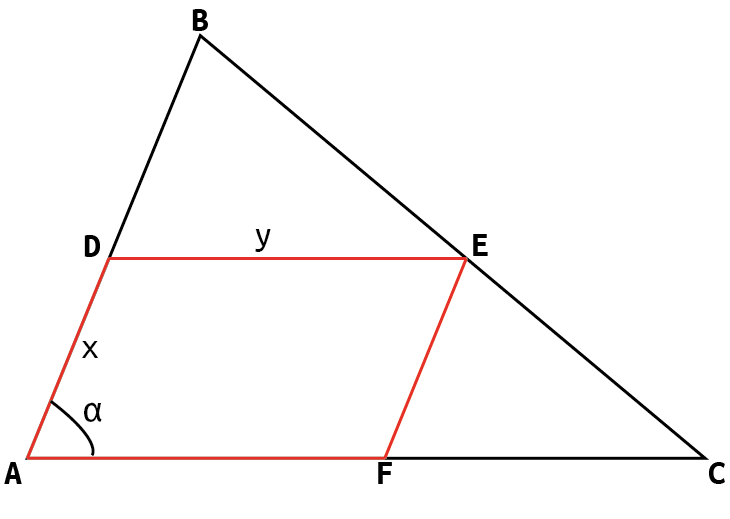
\includegraphics[scale=0.5]{pics/geom_evklid.png}
        \caption{Задача Евклида}
    \end{figure}

    Пусть $x = AD,\ y = AF, \alpha = \angle DAF$. Выпишем площадь параллелограмма: $S_{ADEF} = \frac{1}{2} xy \sin \alpha$. Площадь $\Delta ABC$ можно выразить несколькими способами
    \begin{equation*}
        \frac{1}{2} AB\ AC\ \sin \alpha = S_{ABC} = S_{ADEF} + \frac{1}{2} (AB - x) y \sin \alpha + \frac{1}{2} (AC - y) x \sin \alpha
    \end{equation*}
    Тогда получим задачу
    \begin{equation*}
        \begin{cases}
            AB \cdot y + AC \cdot x = AB \cdot AC\\
            xy \rightarrow \text{max}
        \end{cases}
    \end{equation*}
    Нужно найти максимум функции $f(x) = -x^2 \frac{AC}{AB} + AC \cdot x$ (\textbf{узнали задачу ?}). Решаем
    \begin{equation*}
        f^{'}(x) = -2x \frac{AC}{AB} + AC = 0 \Rightarrow x = \frac{AB}{2},\ y = \frac{AC}{2}
    \end{equation*}
    Таким образом мы решили задачу Евклида и нашли, что параллелограмм наибольшей площади вписан в треугольник, если его стороны равны половине сторон треугольника.
\end{example}
Finally, физика!
\begin{example}
    Тело массой $m$, находящееся на горизонтальной поверхности, испытывает действие постоянной по модулю силы $F$. Угол $\alpha$ между вектором силы и горизонтом можно изменять. Определить максимально возможное ускорение тела. Коэффициент трения между телом и поверхностью равен $\mu$.

    \begin{figure}[h!]
        \centering
        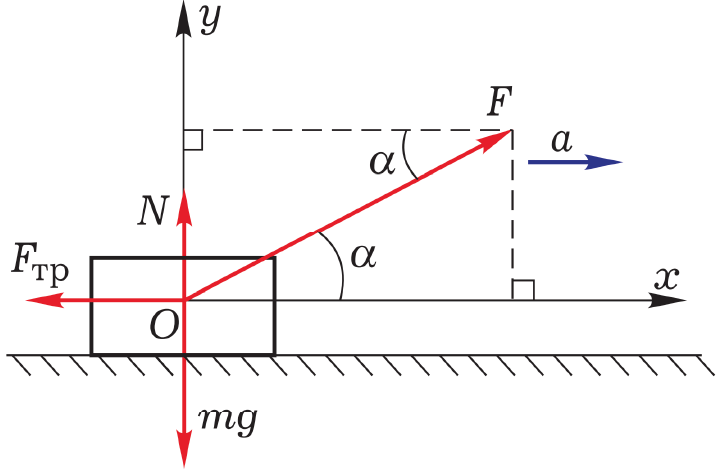
\includegraphics[scale=0.7]{pics/phys_force_extr.png}
        \caption{Рисунок к задачке}
    \end{figure}

    Второй закон Ньютона в проекции по осям
    \begin{eqnarray*}
        OX: && F \cos \alpha - \mu N = m a\\
        OY: && F \sin \alpha  +N - mg = 0
    \end{eqnarray*}
    Ускорение $a = \frac{F}{m} \bigl(\cos \alpha + \mu \sin \alpha \bigr) - \mu g$. Приравняем к нулю производную по углу
    \begin{equation*}
        \frac{da}{d\alpha} = \frac{F}{m} \bigl(-\sin \alpha + \mu \cos \alpha \bigr) = 0 \Rightarrow \tan \alpha_{0} = \mu
    \end{equation*}
    А значит 
    \begin{equation*}
        a_{\text{max}} = \frac{F}{m} \sqrt{1 + \mu^2} - \mu g
    \end{equation*}
    \textbf{почему это максимум?}
\end{example}
\subsection{Ряд Тейлора, детка}
Зачастую значение функции приходится считать приближенно в какой-либо точке $x_0$ в рамках заданных условий задачи. Например, в задачах геометрической оптики используют приближение малых углов отклонения. Исследовать поведение функции в окрестности точки $x_0$ можно с помощью ряда Тейлора.
\begin{definition}
    \textbf{Ряд Тейлора} $n$ раз непрерывно-дифференцируемой функции $f(x)$ в точке $x_0$ - это ряд вида
    \begin{equation*}
        f(x) = \sum_{k = 0}^{n}\frac{f^{(k)}(x_0)}{k!} (x - x_0)^k + R_{n+1}(x),
    \end{equation*}
    где $R_{n+1}(x)$ - остаточный член, который стремится к нулю при $x \to x_0$.
\end{definition}

Распишим основные функции в ряд Тейлора в окрестности точки $x_0 = 0$. Такое разложение вблизи $0$ \textbf{рядом Маклорена}:
\begin{itemize}
    \item $e^{x} = \sum_{k = 0}^{\infty} \frac{x^k}{k!} \approx 1 + x$
    \item $\sin x = \sum_{k = 0}^{\infty} \frac{x^{2k + 1}}{(2k + 1)!} \approx x - \frac{x^3}{3}$
    \item $\cos x = \sum_{k = 0}^{\infty} \frac{(-1)^k x^{2k}}{(2k)!} \approx 1 - \frac{x^2}{2}$
\end{itemize}

\begin{example}[Формула Эйлера]
    Докажем одну из самых красивых формул математики
    \begin{equation*}
        e^{ix} = \cos x + i \sin x
    \end{equation*}
    Разложим экспоненту в ряд Маклорена
    \begin{multline*}
        e^{ix} = \sum_{k = 0}^{\infty} \frac{(ix)^k}{k!} = \{i^2 = -1, i^3 = -i, \dots \}= \sum_{k = 0}^{\infty} \frac{x^{2k}}{(2k)!} + i \sum_{k = 0}^{\infty} \frac{x^{2k + 1}}{(2k + 1)!} = \\
        = \cos x + i \sin x
    \end{multline*}
    Эта формула будет встречаться во множестве физических задач, особенно в квантовой механике, где она используется для описания волновых функций частиц.
\end{example}
\newpage
\section{Интеграл}
\subsection{С чем его едят?}
\subsection{Вновь движемся, вопрос куда...}
\subsection{Интеграл, как площадь под графиком функции}
\subsection{Формула Ньютона-Лейбница}
\subsection{Джедайство интеграла}
\subsection{Интегрирование по углам}
\section{Колебания и дифференциальные уравнения}
\epigraph{\textsf{May the force be with you.}}{\texttt{Everybody from SW.}}
Перейдем к кульминации всего курса - составлению дифференциальных уравнений (уравнения на функцию, где фигурирует ее производная), которые являются неотъемлемой частью познания физических законов. Не будем перегонять из пустого в порожнее!
\subsection{Формула Циолковского}
\begin{figure}[h!]
    \centering{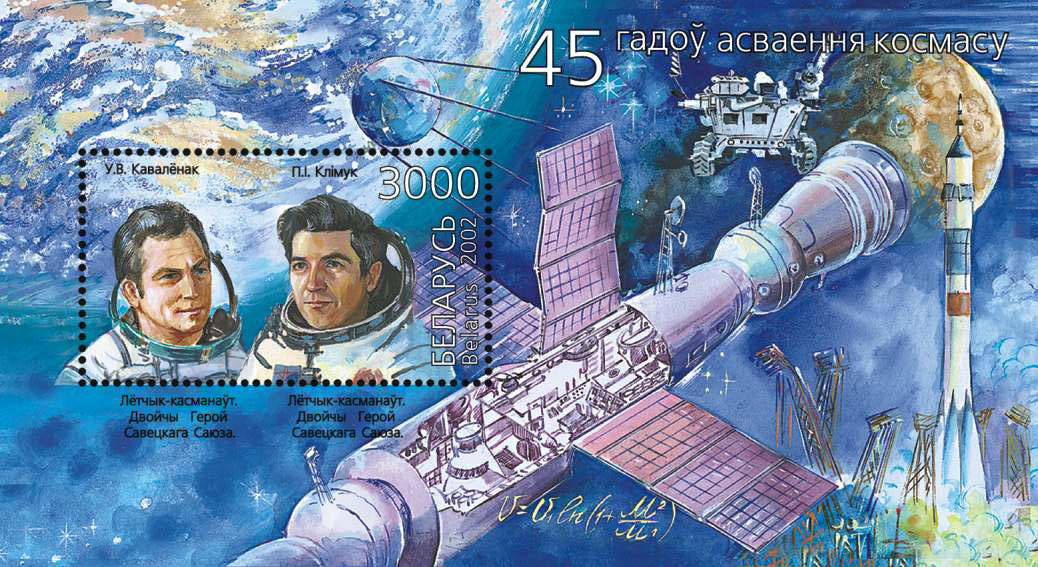
\includegraphics[scale=0.2]{pics/rocket.jpg}}
    \caption{Уравнение Циолковского на марке}
\end{figure}

Рассмотрим движение ракеты в космосе.
Сначала пренебрежём всеми внешними силами, действующими на ракету. Основными параметрами, характеризующими ракету и её двигатель, являются: $\boldsymbol{u}_0$ — скорость истечения газов из сопла ракеты относительно корпуса ракеты, для простоты считаем её постоянной, $M_0$ — исходная масса ракеты с горючим, $M_{\text{к}}$ — конечная масса ракеты после выгорания всего горючего.

Ракета имеет скорость $v$, массу $M$ в момент времени $t$. Выбрасывается топливо массы $\Delta M$ со скоростью $u_0$. Импульс сохраняется, тогда 
\begin{equation*}
    Mv = (M - \Delta M)(v + \Delta v) + \Delta M (v + u_0)
\end{equation*}

Тогда получим дифференциального уравнение 1-го порядка (фигурирует производная 1-ой степени)
\begin{equation*}
    M\Delta v =  - \Delta M u_0 \Rightarrow v(t) = - u_0 \int_{M_0}^{M_\text{к}} \frac{dM}{M}
\end{equation*}
Этот сделан предварительно перейдя к дифференциалам. Итого
\begin{equation*}
    v = u_0 \ln \Bigl(\frac{M_0}{M_{\text{к}}} \Bigr)
\end{equation*}
Таким образом, скорость ракеты увеличивается с уменьшением массы ракеты!!! Именно поэтому мы грузим топливо в ракеты, а не просто запускаем их из, например, рогатки.
\subsection{Почему Коши оказался в диффурах?}
Теперь зададимся вопросом - почему дифференциальные уравнения (вообще любые) имеют решения при должном числе условий, наложенных на функцию? Оказывается, что ответ на этот вопрос был дан довольно-таки давно. Задачи, где дано дифференциальное уравнение и условие на функцию, называют \textit{задачами Коши}. Например, уравнение Циолковского
\begin{equation*}
    \begin{cases}
        \frac{dv}{dM}= - \frac{u_0}{M}\\
        v(M = M_0) = 0
    \end{cases}
\end{equation*}

Так оказывается, что такие задачи \textbf{всегда} имеют решение!
\begin{theorem}(Теорема о разрешимости задачи Коши)
    Пусть есть поставленная задача Коши на отрезке
    \begin{equation*}
        \begin{cases}
            y^{'} = f(x,y),\ x \in (x_0, a]\\
            y^{'}(x_0) = y^{0}
        \end{cases}
    \end{equation*}
    Тогда, если функция $f(x,y)$ удовлетворяет (\dots \textbf{куча условий} \dots), то решение \textbf{существует} и \textbf{единственно}.
\end{theorem}
Подробнее об этом вам расскажут в университете, поэтому на этом мы внимание заострять не будем. Зато теперь мы решаем дифференциальные уравнения законно!
\subsection{Математический маятник: чем больше тел, тем сложнее путь}
Теперь попробуем решить задачу для колебания математического маятника.
\begin{figure}[h!]
    \centering{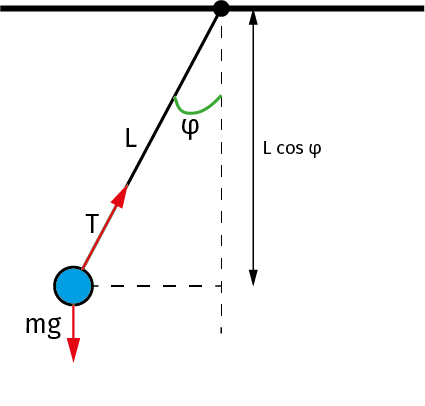
\includegraphics[scale = 1]{pics/mat_mayatnik.png}}
    \caption{Математический маятник.}
\end{figure}

Поступим следующим образом: запишем полную энергию системы а потом уже найдем силу, действующую на груз. Сначала перейдем к углу отклоения $\phi$ и выразим все через него. Таким образом
\begin{equation*}
    y = -L\cos \phi,\ x = L \sin \phi
\end{equation*} 

Полная энергия системы равна
\begin{equation*}
    W = \frac{m L^2 \dot{\phi}^2}{2} - mgL \cos \phi
\end{equation*}
Теперь запишем теорему, которая нам пригодится
\begin{theorem}(Связь силы и поля)
    Равнодействуйющая всех сил, действующих на систему, связаны с потенциальной энергией $U$ следующим соотношением
    \begin{equation*}
        F_x = -\frac{\partial U}{\partial x},\ F_y = -\frac{\partial U}{\partial y},\ F_z = -\frac{\partial U}{\partial z} \Rightarrow \vec{F} = - \nabla U
    \end{equation*}
    где значок $\nabla$ - называется \textbf{наблой}, и под собой подразумевает $\nabla = \{\frac{\partial}{\partial x},\frac{\partial}{\partial y}, \frac{\partial}{\partial z} \}$
\end{theorem}
\begin{proof}
    Так как $dA = (\vec{F}, d \vec{r})$, а $dA = - dU$, то 
    \begin{equation*}
        dU = -(\vec{F}, d \vec{r}) = - F_x dx - F_y dy - F_z dz \Rightarrow F_{\alpha_i} = - \frac{\partial U}{\partial \alpha_i},\ \alpha_i = {x, y, z}
    \end{equation*}
    И тогда $\vec{F} = - \nabla U$
\end{proof}
Так как мы "сидим"\ в угловых координатах, то изменение положения маятника будет происходить по дуге. Тогда
\begin{equation*}
    m a_{\text{ц.с.}} = m l \ddot{\phi} = - \frac{\partial U}{L \partial \phi} = mg \frac{\partial \cos \phi}{\partial \phi } = - mg \sin \phi
\end{equation*}

Таким образом
\begin{equation*}
    \ddot{\phi} = - \frac{g}{L} \sin \phi
\end{equation*}
Если воспользоваться допущением, что угол отклонения $\phi$ мал, то мы получим
\begin{equation*}
    \ddot{\phi} = - \frac{g}{L} \phi \Rightarrow \ddot{\phi} + \omega^2 \phi = 0,\ \omega = \sqrt{\frac{g}{L}}
\end{equation*}
Решением такого дифференциального уравнения являются гармонические функции
\begin{equation*}
    \phi(t) = A \cos (\omega t) + B \sin (\omega t)
\end{equation*}
где $A$ и $B$ можно найти из начальных условий. 

Данную задачу можно было решить по другому, если бы мы спроецировали силу тяжести на ось, перпендикулярную нити
\begin{equation*}
    m a_{\tau} = m l \ddot{\phi}  = - mg\sin \phi
\end{equation*}

\break

\subsection{Гармонический осциллятор}
Рассмотрим еще один известнейший маятник - пружинный. 

\begin{figure}[h!]
    \centering{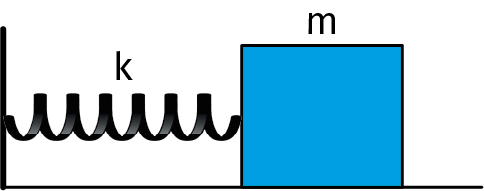
\includegraphics[scale=0.7]{pics/pruz_mayatnik.png}}
    \caption{Пружинный маятник.}
\end{figure}

Запишем второй закон Ньютона при отклонении на малую величину $x$
\begin{equation*}
    m\ddot{x} = \Bigl(kx_0 - k(x + x_0) \Bigr) = - kx \Rightarrow \ddot{x} + \omega^2 x = 0,\ \omega = \sqrt{\frac{k}{m}}
\end{equation*}

Давайте запишем полную энергию маятника
\begin{equation*}
    W = \frac{m \dot{x}^2}{2} + \frac{kx^2}{2}
\end{equation*}
\begin{prac}
    Получи дифференциальное уравнение для колебаний способом, как для математического маятника.
\end{prac}
Как ты видишь, теперь у нас есть возращающая сила в системе (сила упругости), которая пропорциональна отклонению. Оказывается, что такое поведение характерно для очень многих систем, особенно в акустических и иных средах, где молекулы начинают колебаться относительно положения равновесия.

Также, предметом изучения может служить в рамках гармонического осциллятора могут служить поведения вакуума и света в различных средах, но это уже вопросы квантовой механики, о которых мы не рассказываем в этом курсе.
\subsection{Фазовая плоскость и фазовая траектория}
\begin{definition}
    \textbf{Фазовая траектория} - график импульса от координаты (1D случай).
\end{definition}
Попробуем вообразить как фазовая плоскость будет выглядеть для разных задач.
\begin{example}(Пружинный маятник)
    Для него мы только что получили значение координаты
    \begin{equation*}
        x = A \cos(\omega t + \phi_0)
    \end{equation*}
    Импульс же
    \begin{equation*}
        p = m \dot{x} = -Am\omega \sin(\omega t + \phi_0)
    \end{equation*}
    Но таким образом
    \begin{equation*}
        \frac{x^2}{A^2} + \frac{p^2}{(A m \omega)^2} = 1
    \end{equation*}
    А это уравнение эллипса! Это означает, что для гармонических колебаний фазовая траектория замкнутая и имеет эллиптическую форму. Это действительно должно быть так, так как полная энергия системы сохраняется и переход из потенциальной в кинетическую. Тоже самое будет изображено на фазовой траектории.
\end{example}

\begin{prac}
    Нарисовать фазовую траекторию математического маятника (с приближением малых углов и без него).
\end{prac}

\textbf{Если успеем, то расскажу еще про колебания с затуханием + фазовый портрет.}

\newpage
\thispagestyle{empty}
\renewcommand{\thesubsection}{\roman{subsection}}
\setcounter{subsection}{0}
\markboth{Задачи}{Задачи}
\addcontentsline{toc}{section}{Задачи}
\section*{Задачи}

\subsection*{Нулевое занятие. Функции одной переменной}
\addcontentsline{toc}{subsection}{Функции одной переменной}
\begin{enumerate}
    \item По графику квадратного трехчлена $y = ax^2 + bx + c$ определить знаки коэффициентов.
    \item Упростить выражения:
    \begin{enumerate}
        \item $\cos (x - y) - \sin x \sin y$
        \item $\frac{1}{2} \cos x - \sin(\frac{\pi}{6} + x)$
    \end{enumerate}
    \item Построить графики функций:
    \begin{enumerate}
    \begin{minipage}{0.5\textwidth}
        \item $y = \cos (2x + \frac{\pi}{2})$
        \item $y = \tan (x + \frac{\pi}{3})$
        \item $y = \sin (2x - \frac{\pi}{4})$
    \end{minipage}
    \begin{minipage}{0.5\textwidth}
        \item $y = \log_2 x$
        \item $y = \log_3 (x - 1)$
        \item $y = \log_{10} (x + 2)$
    \end{minipage}
    \end{enumerate}
    \item Докажите тождество: $\frac{\tan \alpha + \tan \beta}{\tan(\alpha + \beta)} + \frac{\tan \alpha - \tan \beta}{\tan(\alpha - \beta)} = 2$
    \item Пользуясь только определением логарифмической функции, вычислить: 
    \begin{enumerate}
    \begin{minipage}{0.5\textwidth}
        \item $\log_2 256$
        \item $\log_4 (2^{2002})$
        \item $\log_3 (27^{15})$
        \item $\log_{27} (3^{99})$
    \end{minipage}
    \begin{minipage}{0.5\textwidth}
        \item $\ln(e^{2003})$
        \item $2^{\log_2 5}$
        \item $e^{\ln 2003}$
        \item и т.д.
    \end{minipage}
    \end{enumerate}
    \item $\boldsymbol{*}$ Доказать формулу $\log_a x = \frac{\log_b x}{\log_b a}$ для любых $a, b, x > 0$, $a \neq 1, b \neq 1$.
    \item $\boldsymbol{*}$ Доказать, что $\log_a x = \frac{1}{\log_x a}$ при $a >0, a\neq 1, x>0, x \neq 1$.
    \item $\boldsymbol{**}$ Натуральный логарифм числа $x$ можно приближённо вычислить, даже если на калькуляторе нет кнопок, кроме кнопки извлечения квадратного корня: надо десять раз нажать на эту кнопку, из результата вычесть единицу, а разность умножить на $1024$. Попробуйте объяснить, почему этот способ работает, если число $x$ не слишком большое и не слишком близко к нулю.
    
\end{enumerate}
\newpage
\thispagestyle{empty}
\subsection*{Производная}
\addcontentsline{toc}{subsection}{Производная}
\begin{enumerate}
    \item По графику функции $y = f(x)$ нарисовать график функции ее производной $y = f^{'}(x)$ (см.вниз\footnote{придумай график сам и нарисуй})
    \item Найдите производные функций по определению, используя предел:
    \begin{enumerate}
    \begin{minipage}{0.5\textwidth}
        \item $y(x) = C = const$
        \item $y(x) = x$
        \item $y(x) = x^2 + 10$ в точке $x = 3$
    \end{minipage}
    \begin{minipage}{0.5\textwidth}
        \item $y(x) = x^3$ в точке $x = 5$
        \item $y(x) = \frac{1}{x}$ в точке $x = 1$
        \item $y(x) = \sqrt{x}$
    \end{minipage}
    \end{enumerate}
    \item Вычислите производные:
    \begin{enumerate}
    \begin{minipage}{0.5\textwidth}
         \item $y(x) = 2 \sqrt[3]{x^2} - \frac{3}{\sqrt{x}}$
        \item $y(x) = \sin x - \cos x$
        \item $y(x) = \tg x - \ctg x$
        \item $y(x) = \cos^2 x \cdot x^2$
    \end{minipage}
    \begin{minipage}{0.5\textwidth}
        \item $y(x) = e^{2x} \sin x$
        \item $y(x) = \frac{x^2 - 2}{\sqrt{x^2 + 1}}$
        \item $y(x) = \sin x \cos x \cdot x $
        \item $y(x) = \sin [ \sin [\sin x]]$
    \end{minipage}
    \end{enumerate}
    \item Написать формулы, задающие координаты точки, равномерно движущейся по окружности, как функции времени. Найти производные этих функций. Что характеризуют эти производные? Как увидеть из полученных формул, что скорость движения направлена по касательной к окружности?
    \item Найти ток в цепи с зарядом $q = A \cos (\alpha e^{-\omega t})$. Когда этот ток максимален?
    \item $\boldsymbol{*}$ Показать, что $\ln x = \lim_{n \rightarrow \infty} n (x^{1/n} - 1)$
    \item $\boldsymbol{*}$ Даны две точки $A$ и $B$ по одну сторону от прямой $l$. Требуется найти на $l$ такую точку $D$, чтобы сумма расстояний от $A$ до $D$ и от $B$ до $D$ была наименьшей.
    \item $\boldsymbol{*}$ Две среды разделены плоской границей. Луч света, идущий из точки, лежащей по одну сторону границы, в точку, лежащую по другую сторону, избирает путь, требующий наименьшего времени. Что это за путь, если скорость движения в указанных средах равна $v_1$ и $v_2$ соответственно?
\end{enumerate}
\newpage
\thispagestyle{empty}
\subsection*{Полезные применения производной. Ряд Тейлора.}
\addcontentsline{toc}{subsection}{Полезные применения производной. Ряд Тейлора.}
\paragraph{Полезные применения производной}
\begin{enumerate}
    \item Точка А движется согласно уравнениям $x_1 = 2t, y_1 = t$, а точка В – согласно уравнениям $x_2 = 10-t, y_2 = 2t$ ($x, y$ – в метрах, $t$ – в секундах). Определить расстояние $S$ между этими точками в момент их максимального сближения. Оба движения в одной плоскости,  – координаты точек в прямоугольной системе координат в этой плоскости
    \item К источнику электрической энергии с ЭДС $E$ и внутренним сопротивлением $r$ подключён реостат. Какую наибольшую тепловую мощность можно получить на внешнем участке цепи?
    \item С какой наименьшей скоростью надо бросить мяч, чтобы забросить его на крышу дома высотой $H$ с расстояния $S$ от дома?
    \item $\boldsymbol{*}$ Вписать в круг единичного радиуса прямоугольник наибольшей площади.
    \item $\boldsymbol{*}$ Ядро, летящее со скоростью $v$, распадается на два одинаковыx осколка. Определите максимальный возможный угол $\alpha$ между скоростями одного из осколков и вектором $v$, если при распаде покоящегося ядра осколки имеют скорость $u<v$.
\end{enumerate}
\paragraph{Ряд Тейлора}
\begin{enumerate}
    \item Разложи в ряд Маклорена функции $f(x)$
    \begin{enumerate}
    \begin{minipage}{0.5\textwidth}
        \item $ f(x) = e^{-x} \quad \text{до члена с } x^n$
        \item $f(x) = e^{2x - x^2} \quad \text{до члена с } x^5$
        \item $f(x) = x\sin x \quad \text{до члена с } x^n$
        
    \end{minipage}
     \begin{minipage}{0.5\textwidth}
        \item $ f(x) = e^{-x} \quad \text{до члена с } x^n$
        \item $f(x) = \ln(1 + x) \quad \text{до члена с } x^n$ 
        \item $f(x) = \sqrt{1 + x} \quad \text{до члена с } x^n$
    \end{minipage}
    \end{enumerate}
    \item \textbf{Связать с физикой?}
\end{enumerate}
\newpage
\thispagestyle{empty}
\subsection*{Интегралы}
\addcontentsline{toc}{subsection}{Интегралы}
\begin{enumerate}
    \item Вычислите интеграл $\int x\ dx$ не беря первообразную.
    \item Вычислите определённые интегралы:
    \begin{enumerate}
    \begin{minipage}{0.5\textwidth}
        \item $\displaystyle \int_{0}^{\pi/2} \cos t \, dt$
        \item $\displaystyle \int_{2}^{8} t^4 \, dt$
        \item $\displaystyle \int_{5}^{10} \frac{1}{t} \, dt$
        \item $\displaystyle \int_{-4}^{4} |x| \, dx$
    \end{minipage}
    \begin{minipage}{0.5\textwidth}
        \item $\displaystyle \int_{1}^{2} \sqrt[3]{x} \, dx$
        \item $\displaystyle \int_{0}^{\pi/2} sin(2025x) \, dx$
        \item $\displaystyle \int_{1}^{2} e^x \, dx$
        \item $\displaystyle \int_{2}^{4} 2^x \, dx$
    \end{minipage}
    \end{enumerate}
    \item Вычислите определённые интегралы:
    \begin{enumerate}
    \begin{minipage}{0.5\textwidth}
         \item $\displaystyle \int_{-\pi}^{\pi} \sin^{25} t \, dt$
    \end{minipage}
    \begin{minipage}{0.5\textwidth}
        \item $\displaystyle \int_{0}^{\pi} \cos^{9} t \, dt$
    \end{minipage}
    \end{enumerate}
    \item Вычислите интеграл: $\displaystyle \int xsin(x) \, dx$
    \item Вычислите неопределённые интегралы:
    \begin{enumerate}
    \begin{minipage}{0.5\textwidth}
         \item $\displaystyle \int \frac{3 - x^2}{3 + x^2} dx$
         \item $\displaystyle \int \frac{dx}{(2 + 3x)^{20}}$
         \item $\displaystyle \int \frac{3x + 2}{2x + 3} dx$
         \item $\displaystyle \int \sqrt{1 + \sin 2x} \, dx$
    \end{minipage}
    \begin{minipage}{0.5\textwidth}
        \item $\displaystyle \int 3^x \cdot 5^x dx$
        \item $\displaystyle \int \frac{\sqrt{x^4 + x^{-4} + 2}}{x^3} dx$
        \item $\displaystyle \int \frac{dx}{1 + \cos x}$
        \item $\displaystyle \int \frac{dx}{1 + \sin x}$
    
    \end{minipage}
    \end{enumerate}
    \item Вычислите определённые интегралы:
    \begin{enumerate}
    \begin{minipage}{0.5\textwidth}
         \item $\displaystyle \int_{-\pi}^{\pi} \sin^{25} t \, dt$
    \end{minipage}
    \begin{minipage}{0.5\textwidth}
        \item $\displaystyle \int_{0}^{\pi} \cos^{9} t \, dt$
    \end{minipage}
    \end{enumerate}
    \item Переходя к полярным координатам, вычислить площади, ограниченные следующими кривыми:
    \begin{enumerate}
        \item $(x^2 + y^2)^2 = 2a^2(x^2 - y^2),\quad x^2 + y^2 \ge a^2$
        \item $(x^3 + y^3)^2 = x^2 + y^2, \quad x \ge 0, y \ge 0.$
    \end{enumerate}
    \item Найдите площадь круга $x^2+y^2=r^2$ 
    \begin{enumerate}
        \item Интегрируя по кольцам малой толщины
        \item Интегрируя по полоскам, перпердикулярным оси $x$
    \end{enumerate}
    \item Найдите площадь эллипса несколькими способами $\displaystyle \frac{x^2}{a^2}+\frac{y^2}{b^2}=r^2$.
    \item Зная значения интеграла Пуассона, вычислите:
    \begin{enumerate}
    \begin{minipage}{0.5\textwidth}
        \item $\displaystyle \frac{1}{\sqrt{2\pi\sigma}} \int_{-\infty}^{+\infty} e^{\frac{-(x-m)^2}{2\sigma^2}}\ dx$
        \item $\displaystyle \int_{-\infty}^{+\infty} xe^{-x^2}\ dx$       
    \end{minipage}
    \begin{minipage}{0.5\textwidth}
        \item $\displaystyle \int_{-\infty}^{+\infty} x^2e^{-x^2}\ dx$   
        \item $\boldsymbol{*}$ $\displaystyle \int_{-\infty}^{+\infty} x^ne^{-x^2}\ dx, n \in \mathbb{N}\cup 0$       
    \end{minipage}
    \end{enumerate}
    \item $\boldsymbol{*}$ Покоящееся тело отпускают с высоты $H$. Найдите время падения тела. $\displaystyle g = \frac{GM}{r^2}$
    \item $\boldsymbol{*}$ Два малых шарика  массы $m$ с зарядами $q$ располагаются на горизонтальной гладкой поверхности на расстоянии $L$. Шарики отпускают. Найдите время, через которое расстояние будет равно $L/2$.
    \item $\boldsymbol{*}$ Имеется жидкая планета в форме однородного шара радиуса $R$ и плотности $\rho$. Найти давление в центре планеты, обусловленное гравитационным притяжением.
    \item $\boldsymbol{*}$ В 1866 году Максвелл разработал теорию, которая показывает, как распределены скорости в идеальном газе при равновесии (расспределение Максвелла). Вероятность найти частицу со скоростью в интервале $[v, v+dv]$ равна:
    \[
    p(v, v+dv) = 4\pi v^2 \left( \frac{m}{2\pi kT} \right)^{3/2} \exp \left( \frac{-mv^2}{2kT} \right) dv.
    \]
    Где $m$ - масса частиц, $T$ - температура газа, $k$ - константа Больцмана. Найти:

        1) Наиболее вероятную скорость
        
        2) Среднюю скорость $<v>$      
        
        3) Среднеквадратичную скорость  $\sqrt{<v^2>}$ 
        
        4) Оцените количесво частиц со скоростью от 499 м/с до 501 м/с в кубическом метре воздуха. Концентрация $n = 3 \cdot$ м$^{-3}$, $T = 273K$, $k = 1.38\cdot 10^{-23}$ Дж/К. 
\end{enumerate}
% \subsection*{Диффуры, колебания и фазовые портреты}
\addcontentsline{toc}{subsection}{Диффуры, колебания и фазовые портреты}

\newpage
\thispagestyle{empty}
\markboth{Контрольная работа}{Контрольная работа}
\addcontentsline{toc}{section}{Контрольная работа}
\section*{Контрольная работа}
% \input{tasks/exam.tex}

\end{document}
